\documentclass{article}\usepackage[]{graphicx}\usepackage[]{color}
% maxwidth is the original width if it is less than linewidth
% otherwise use linewidth (to make sure the graphics do not exceed the margin)
\makeatletter
\def\maxwidth{ %
  \ifdim\Gin@nat@width>\linewidth
    \linewidth
  \else
    \Gin@nat@width
  \fi
}
\makeatother

\definecolor{fgcolor}{rgb}{0.345, 0.345, 0.345}
\newcommand{\hlnum}[1]{\textcolor[rgb]{0.686,0.059,0.569}{#1}}%
\newcommand{\hlstr}[1]{\textcolor[rgb]{0.192,0.494,0.8}{#1}}%
\newcommand{\hlcom}[1]{\textcolor[rgb]{0.678,0.584,0.686}{\textit{#1}}}%
\newcommand{\hlopt}[1]{\textcolor[rgb]{0,0,0}{#1}}%
\newcommand{\hlstd}[1]{\textcolor[rgb]{0.345,0.345,0.345}{#1}}%
\newcommand{\hlkwa}[1]{\textcolor[rgb]{0.161,0.373,0.58}{\textbf{#1}}}%
\newcommand{\hlkwb}[1]{\textcolor[rgb]{0.69,0.353,0.396}{#1}}%
\newcommand{\hlkwc}[1]{\textcolor[rgb]{0.333,0.667,0.333}{#1}}%
\newcommand{\hlkwd}[1]{\textcolor[rgb]{0.737,0.353,0.396}{\textbf{#1}}}%
\let\hlipl\hlkwb

\usepackage{framed}
\makeatletter
\newenvironment{kframe}{%
 \def\at@end@of@kframe{}%
 \ifinner\ifhmode%
  \def\at@end@of@kframe{\end{minipage}}%
  \begin{minipage}{\columnwidth}%
 \fi\fi%
 \def\FrameCommand##1{\hskip\@totalleftmargin \hskip-\fboxsep
 \colorbox{shadecolor}{##1}\hskip-\fboxsep
     % There is no \\@totalrightmargin, so:
     \hskip-\linewidth \hskip-\@totalleftmargin \hskip\columnwidth}%
 \MakeFramed {\advance\hsize-\width
   \@totalleftmargin\z@ \linewidth\hsize
   \@setminipage}}%
 {\par\unskip\endMakeFramed%
 \at@end@of@kframe}
\makeatother

\definecolor{shadecolor}{rgb}{.97, .97, .97}
\definecolor{messagecolor}{rgb}{0, 0, 0}
\definecolor{warningcolor}{rgb}{1, 0, 1}
\definecolor{errorcolor}{rgb}{1, 0, 0}
\newenvironment{knitrout}{}{} % an empty environment to be redefined in TeX

\usepackage{alltt}[12pt]
\usepackage{Sweave}
\usepackage{float}
\usepackage{graphicx}
\usepackage{tabularx}
\usepackage{siunitx}
\usepackage{amssymb} % for math symbols
\usepackage{amsmath} % for aligning equations
\usepackage{mdframed}
\usepackage{natbib}
\bibliographystyle{..//bib/styles/gcb}
\usepackage[hyphens]{url}
\usepackage[small]{caption}
\setlength{\captionmargin}{30pt}
\setlength{\abovecaptionskip}{0pt}
\setlength{\belowcaptionskip}{10pt}
\topmargin -1.5cm        
\oddsidemargin -0.04cm   
\evensidemargin -0.04cm
\textwidth 16.59cm
\textheight 21.94cm 
%\pagestyle{empty} %comment if want page numbers
\parskip 7.2pt
\renewcommand{\baselinestretch}{2}
\parindent 0pt
\usepackage{lineno}
\linenumbers
\usepackage{setspace}
\doublespacing

\newmdenv[
  topline=true,
  bottomline=true,
  skipabove=\topsep,
  skipbelow=\topsep
]{siderules}

%cross referencing:
\usepackage{xr}
\externaldocument{regrisk_supp}

%% R Script


\IfFileExists{upquote.sty}{\usepackage{upquote}}{}
\begin{document}
\noindent 
\textbf{\LARGE{Climate change reshapes the drivers of false spring risk across European trees}} 
%\\
%OR \\
%\textbf{\Large{Climate change increases the risk of false springs in European trees}} \\ % Lizzie votes for the first title! Reviewers can ask you to make it more narrow so I would start here and shift to Ben's if requested ... (goal 1: get paper out for review)
%\textbf{\Large{False spring risk increases across European trees in the face of climate change}}


\noindent Authors:\\
C. J. Chamberlain $^{1,2}$, B. I. Cook $^{3}$, I. Morales-Castilla $^{4,5}$ \& E. M. Wolkovich $^{1,2,6}$
\vspace{2ex}\\
\emph{Author affiliations:}\\
$^{1}$Arnold Arboretum of Harvard University, 1300 Centre Street, Boston, Massachusetts, USA; \\
$^{2}$Organismic \& Evolutionary Biology, Harvard University, 26 Oxford Street, Cambridge, Massachusetts, USA; \\
$^{3}$NASA Goddard Institute for Space Studies, New York, New York, USA; \\
$^{4}$GloCEE - Global Change Ecology and Evolution Group, Department of Life Sciences, Universidad de Alcal\'{a}, Alcal\'{a} de Henares, 28805, Spain \\
$^{5}$Department of Environmental Science and Policy, George Mason University, Fairfax, VA 22030; \\
$^{6}$Forest \& Conservation Sciences, Faculty of Forestry, University of British Columbia, 2424 Main Mall, Vancouver, BC V6T 1Z4\\
\vspace{2ex}
$^*$Corresponding author: 248.953.0189; cchamberlain@g.harvard.edu\\

\renewcommand{\thetable}{\arabic{table}}
\renewcommand{\thefigure}{\arabic{figure}}
\renewcommand{\labelitemi}{$-$}
\setkeys{Gin}{width=0.8\textwidth}

\section*{Tables and Figures} 

{\begin{figure} [H]
  -\begin{center}
  -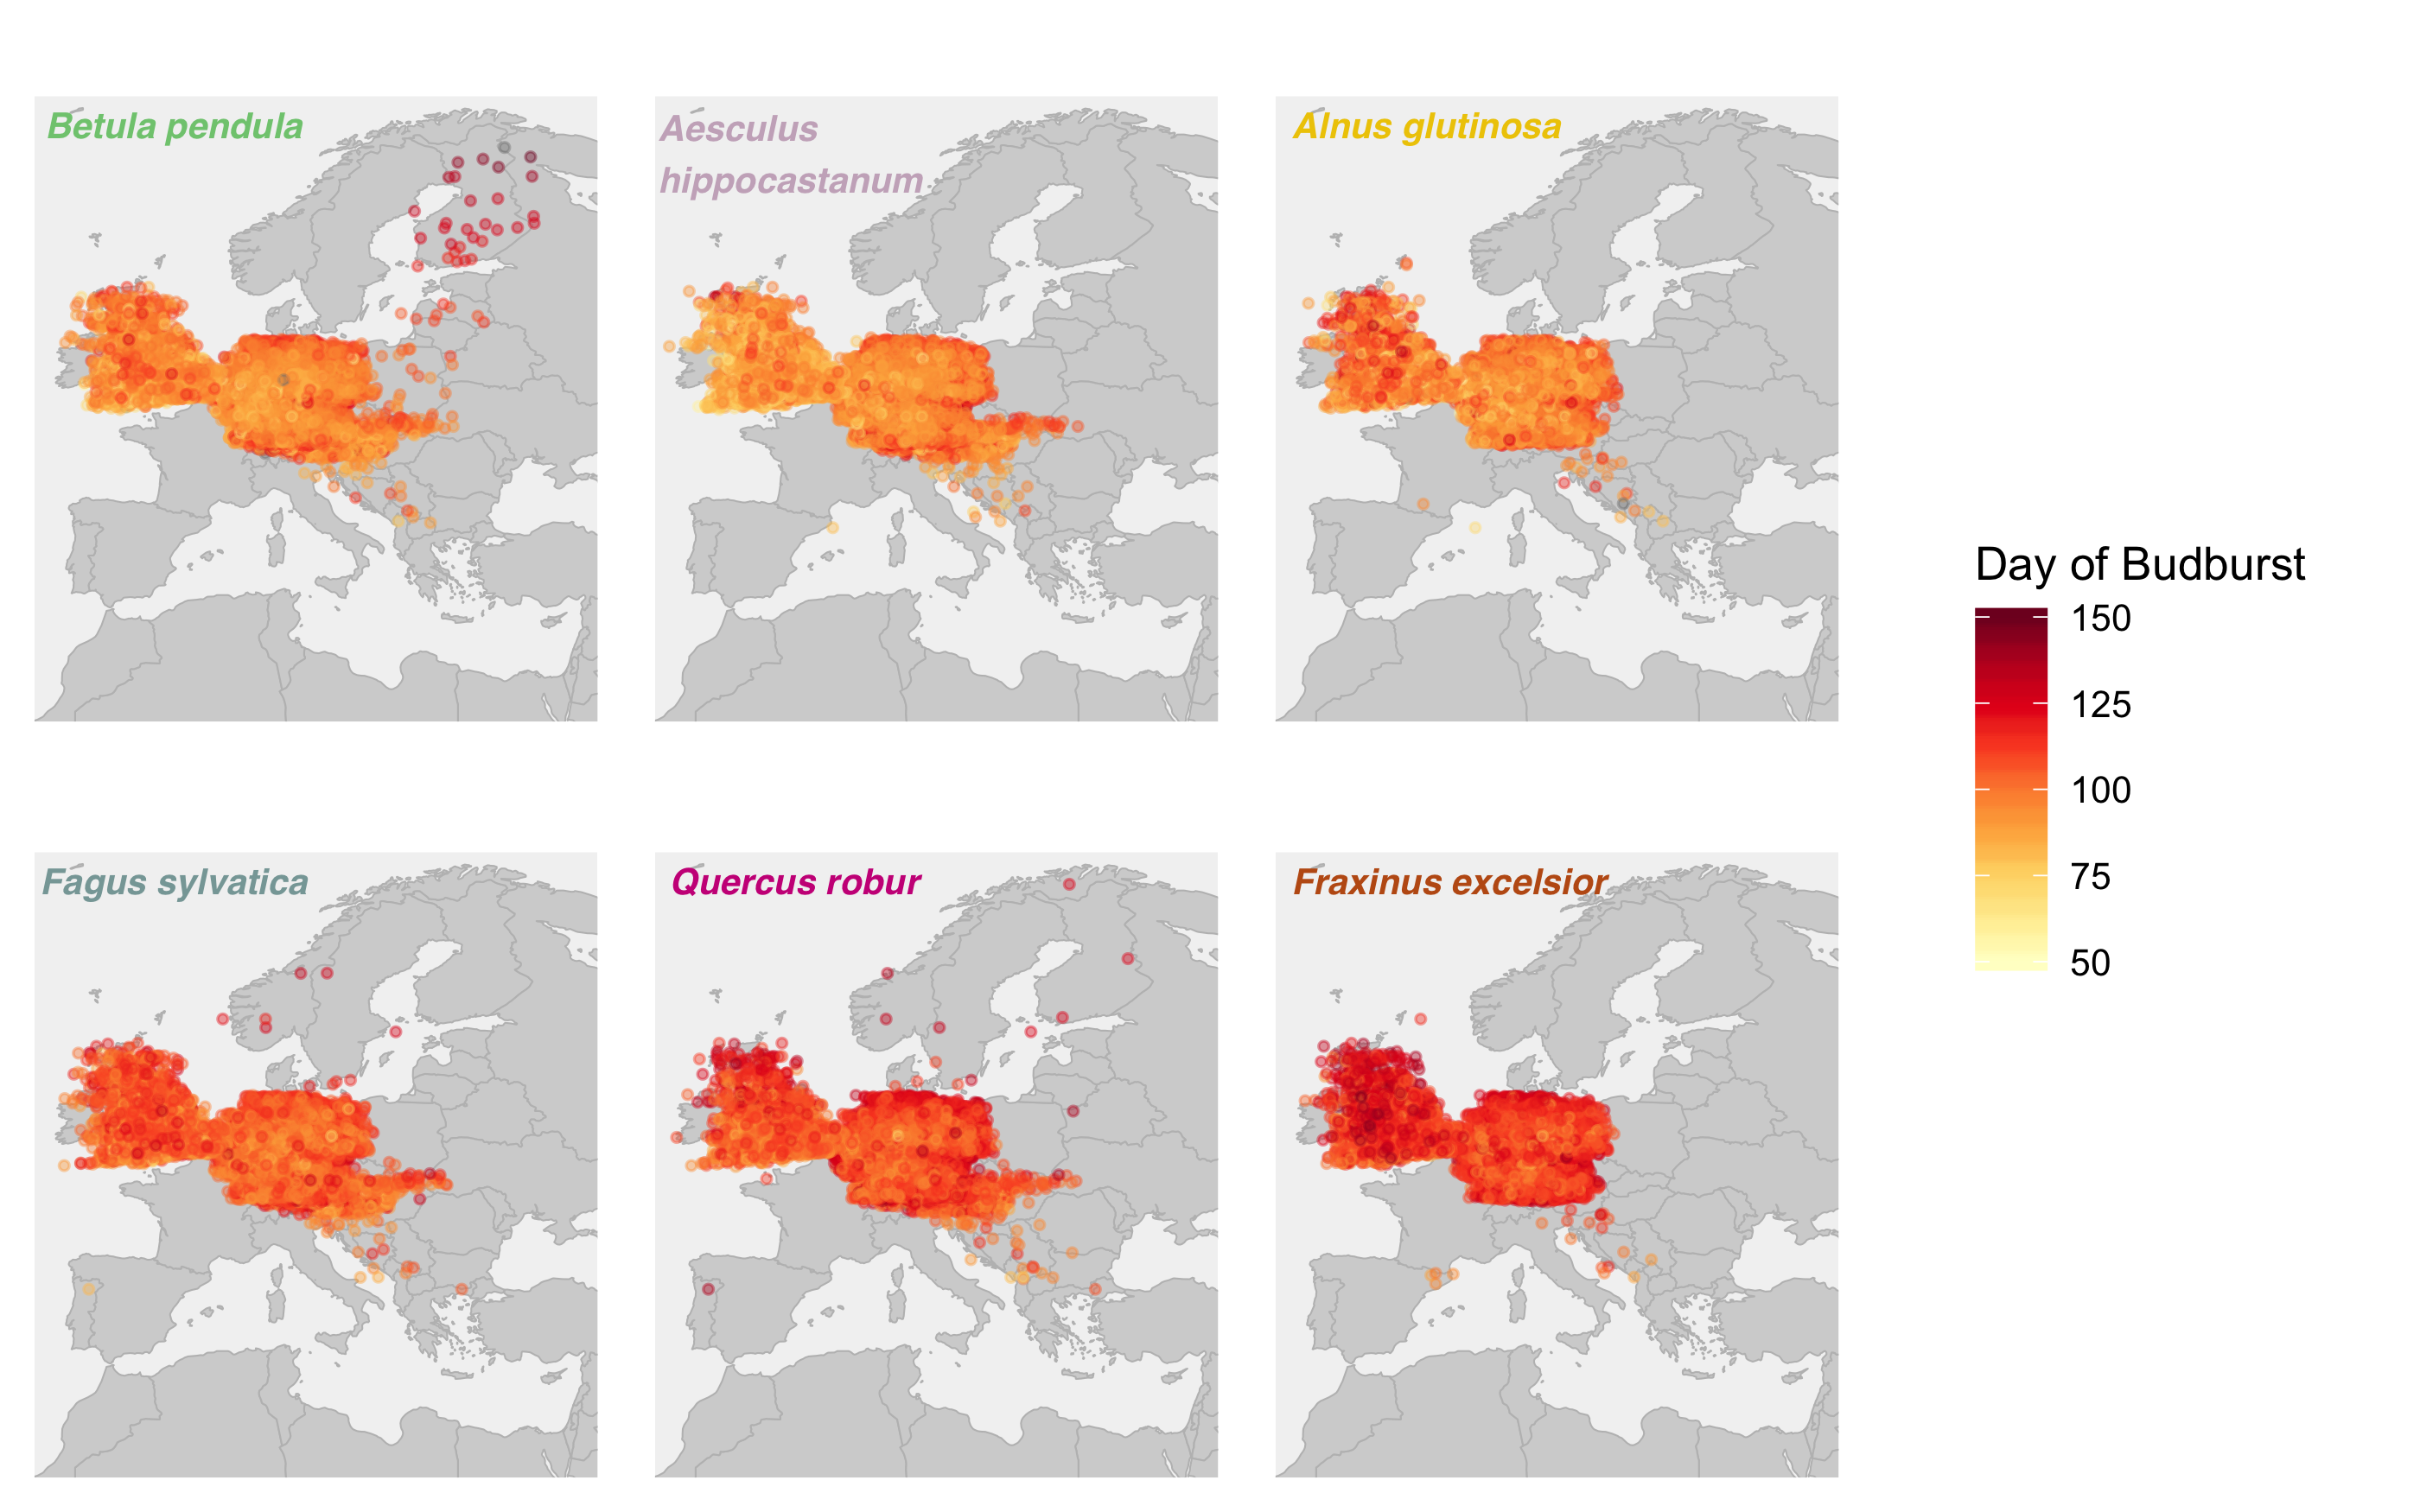
\includegraphics[width=14cm]{..//analyses/figures/BB_base.png}
  -\caption{The average day of budburst mapped by site for each species (ordered by day of budburst starting with \textit{Betula pendula} as the earliest budburst date to \textit{Fraxinus excelsior}). Species names are color-coded to match figures throughout the text. }\label{fig:bbmap}
  -\end{center}
  -\end{figure}}
  
{\begin{figure} [H]
  -\begin{center}
  -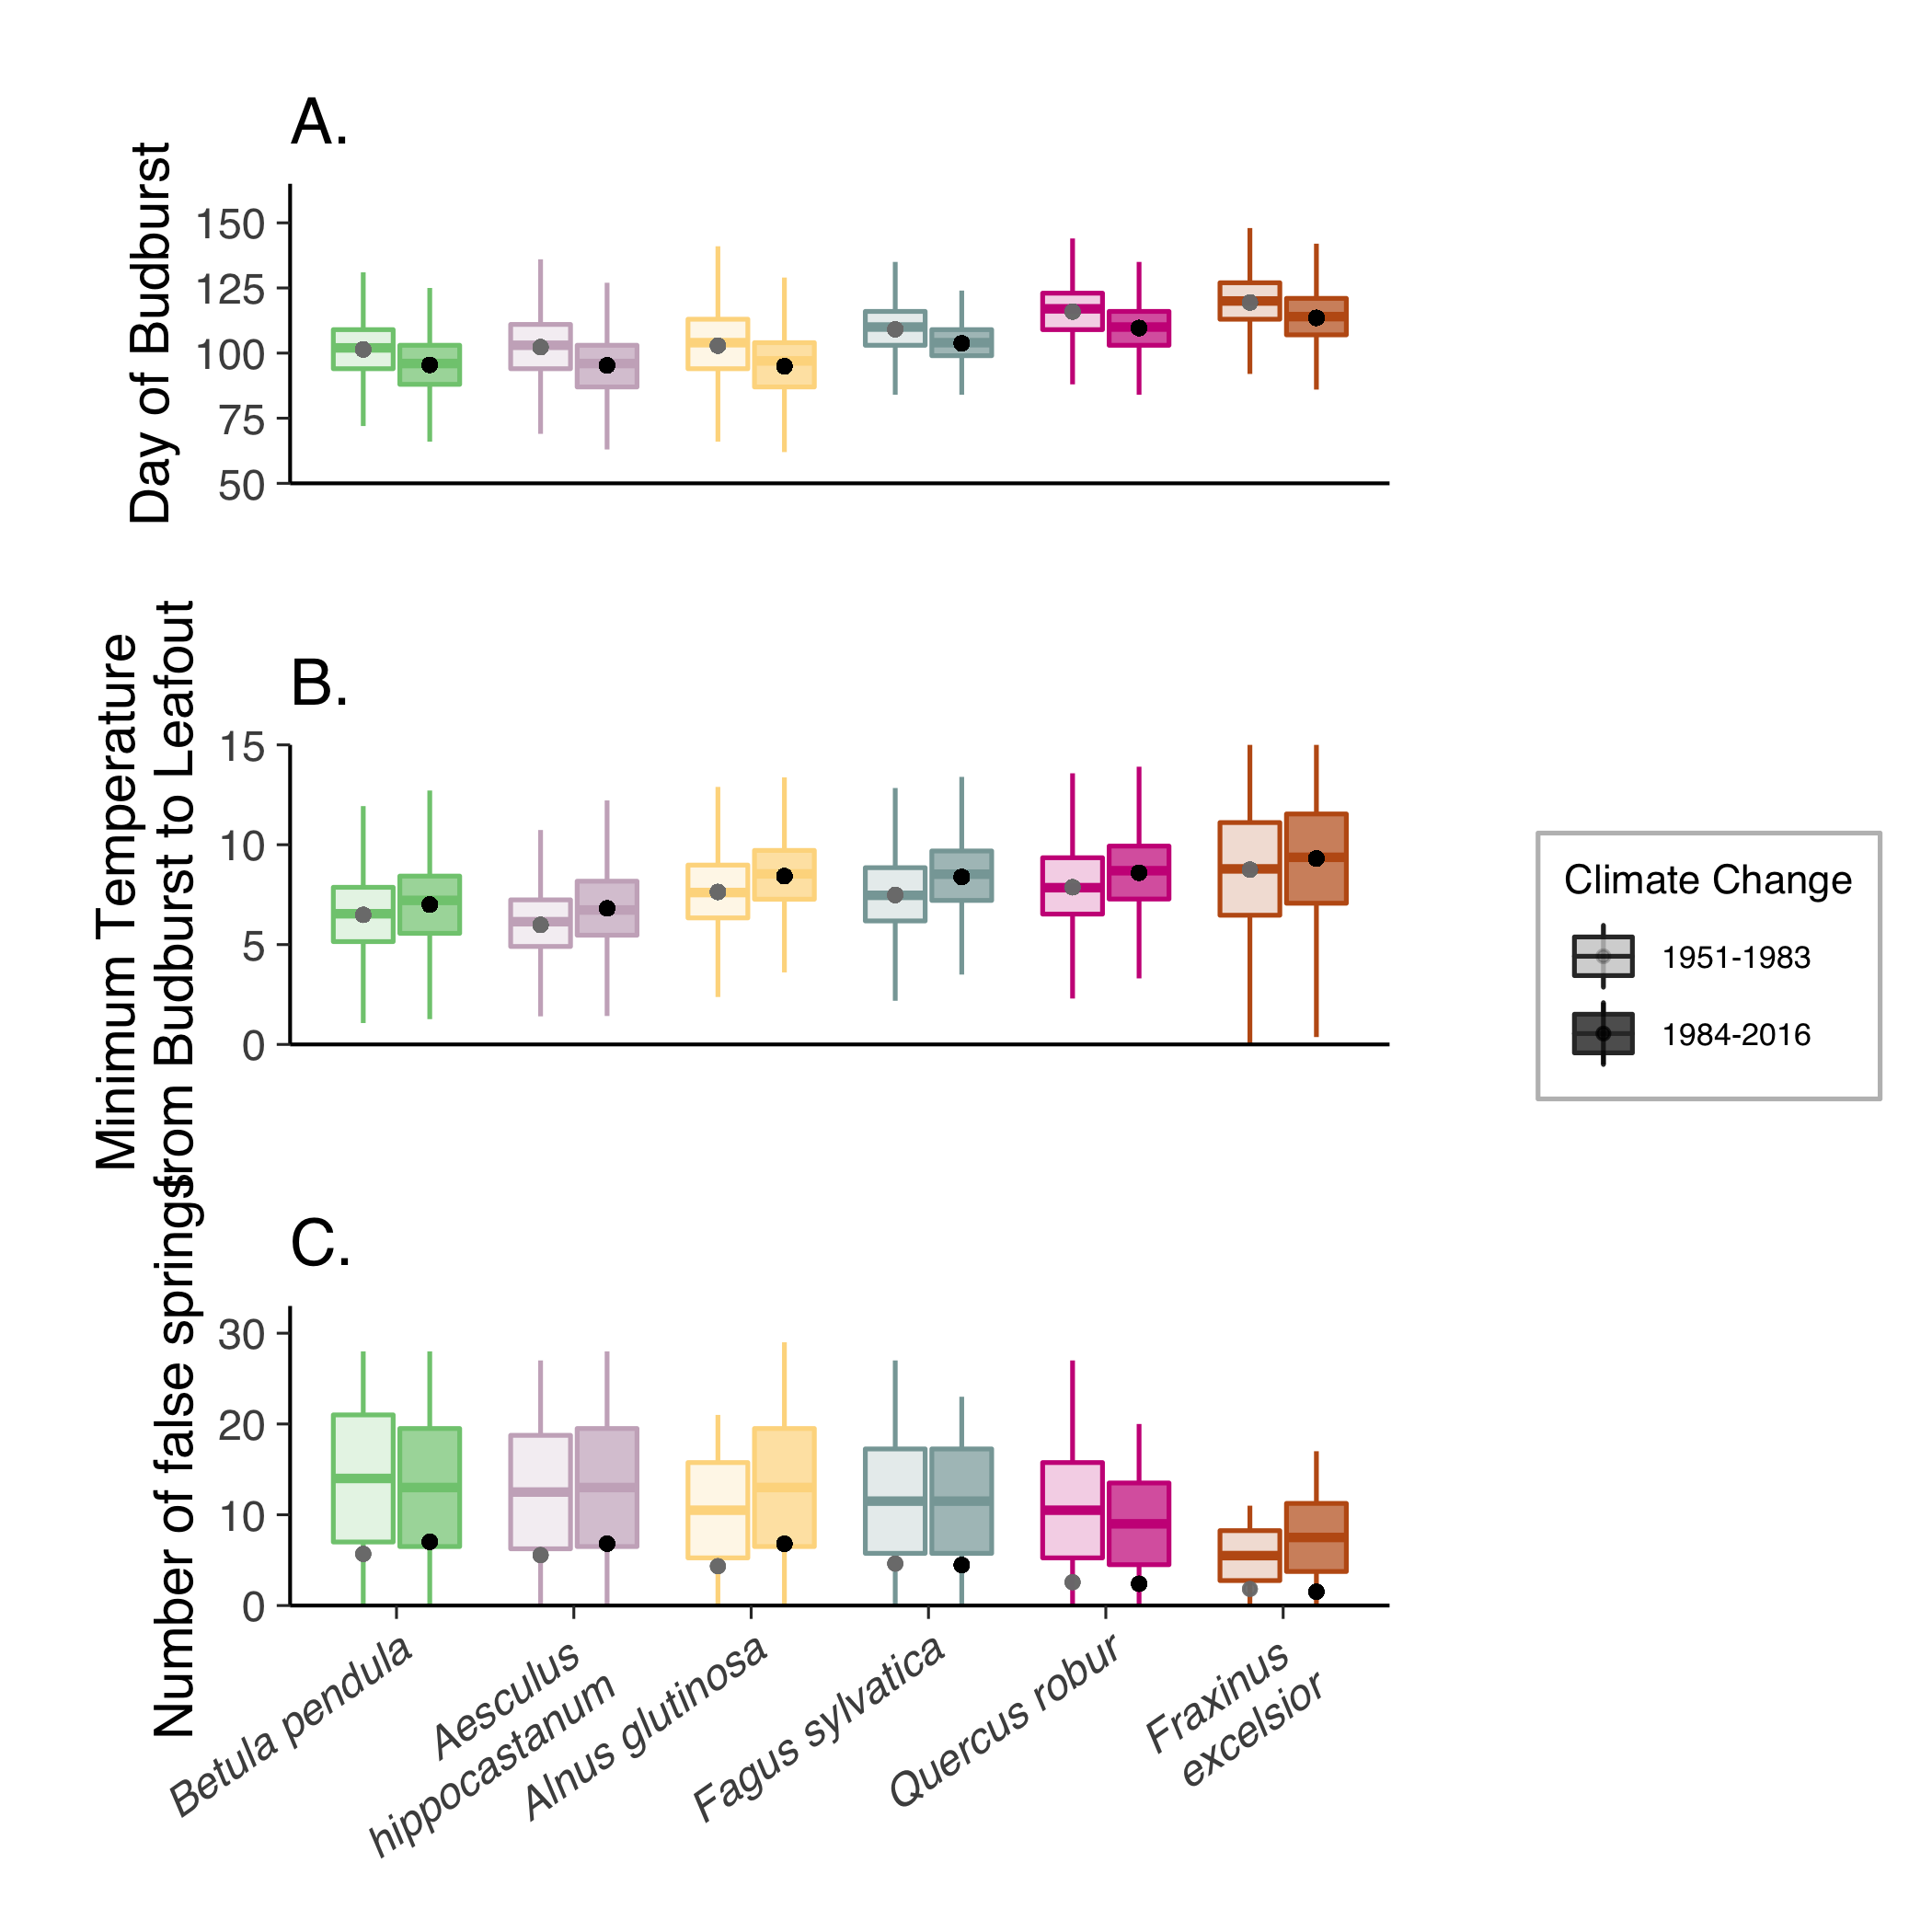
\includegraphics[width=14cm]{..//analyses/figures/Boxplot_BBTminFS_noDots_modests.png}
  -\caption{Day of budburst (\textbf{a}), minimum temperatures between budburst and leafout (\textbf{b}) and number of false springs (\textbf{c}) before and after 1983 across species for all sites. Box and whisker plots show the 25th and 75th percentiles (i.e., the interquartile range) with notches indicating 95\% uncertainty intervals. Dots and error bars overlaid on the box and whisker plots represent the model regression outputs (Tables \ref{tab:simbbmod}-\ref{tab:simpfs}). Error bars from the model regressions indicate 98\% uncertainty intervals but, given the number of sites, are quite small and thus not easily visible (see Tables \ref{tab:simbbmod}-\ref{tab:simpfs}). Species are ordered by day of budburst and are color-coded to match the other figures.  }\label{fig:boxfs}
  % Are you sure the 'notches indicate 95\% uncertainty intervals'? If these are just plots of the RAW data then I am not sure how the box and whisker plots can generate uncertainty.... You generally need a model for that. CJC: These are the error bars from the simple models on top of the box and whisker plots. I can update the language if this is confusing!
  -\end{center}
  -\end{figure}}
  
  
{\begin{figure} [H]
  -\begin{center}
  -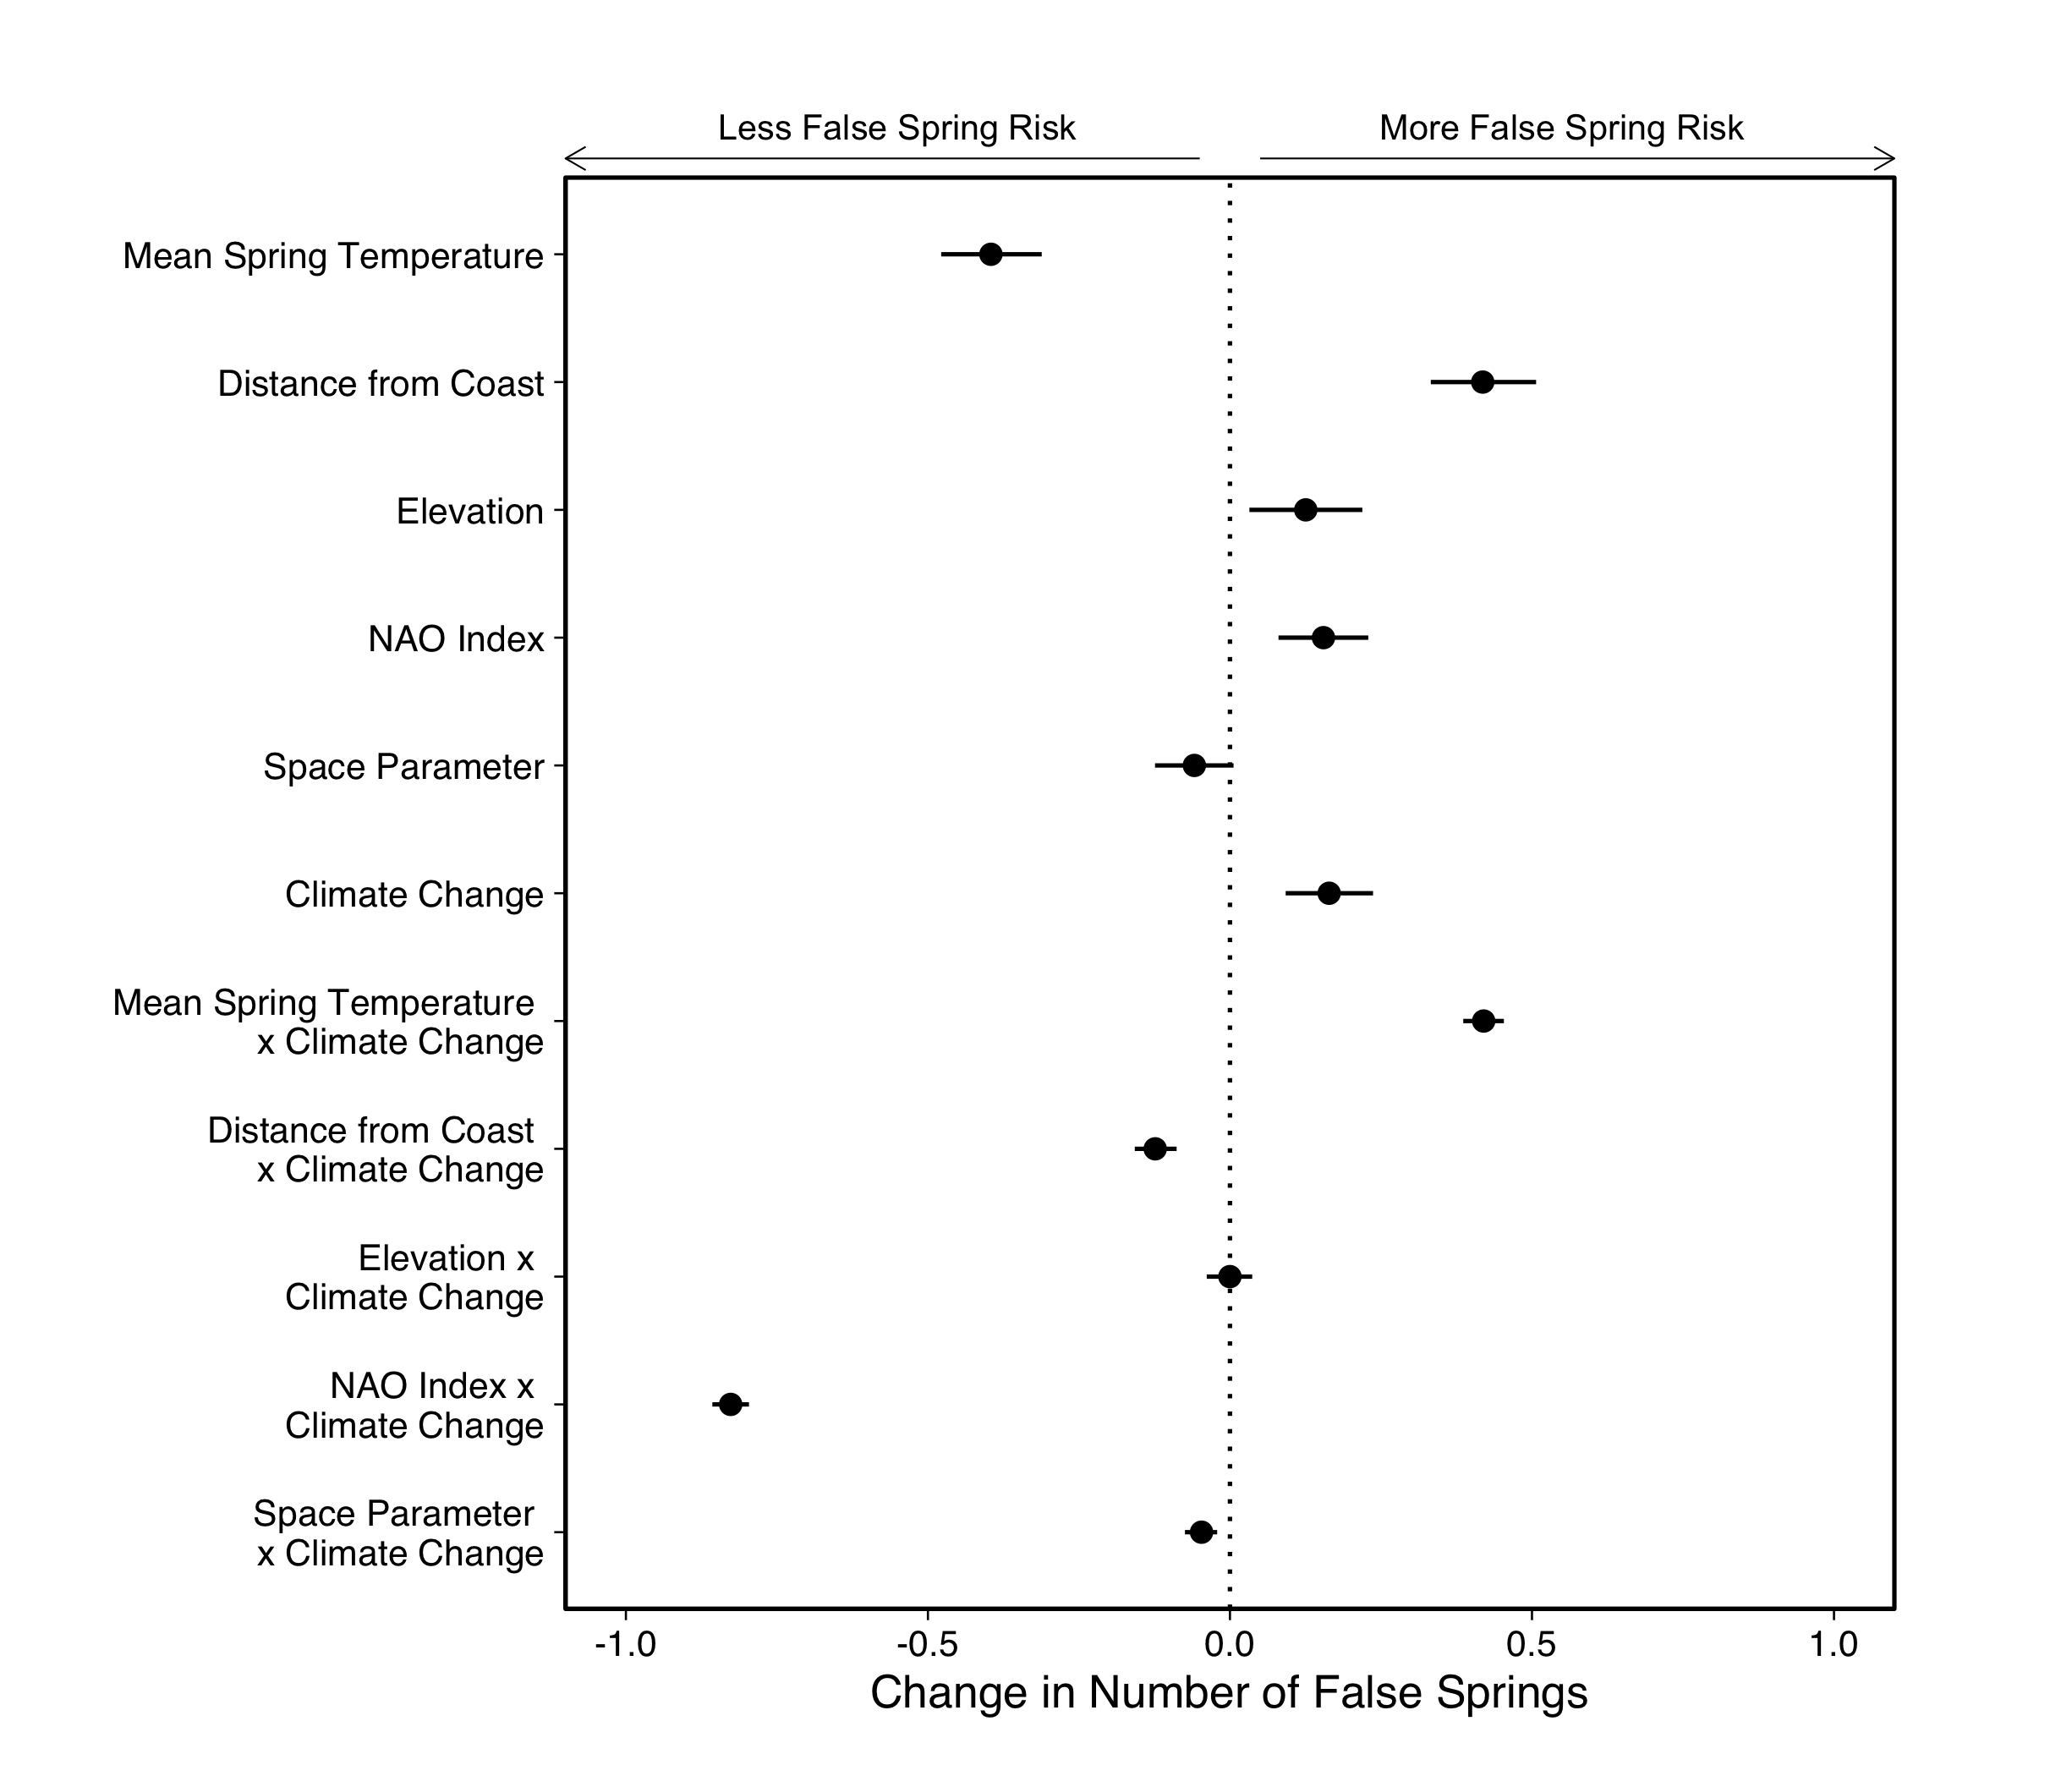
\includegraphics[width=12cm]{..//analyses/figures/model_output_98_orig.png}
  -\caption{Effects of species, climatic and geographical predictors on false spring risk. More positive values indicate an increased probability of a false spring whereas more negative values suggest a lower probability of a false spring. Dots and lines show means and 98\% uncertainty intervals. There were 582,211 zeros and 172,877 ones for false springs in the data. See Table \ref{tab:suppmodorig} for full model output.}\label{fig:maineffects}
  -\end{center}
  -\end{figure}}

  
{\begin{figure} [H]
  -\begin{center}
  -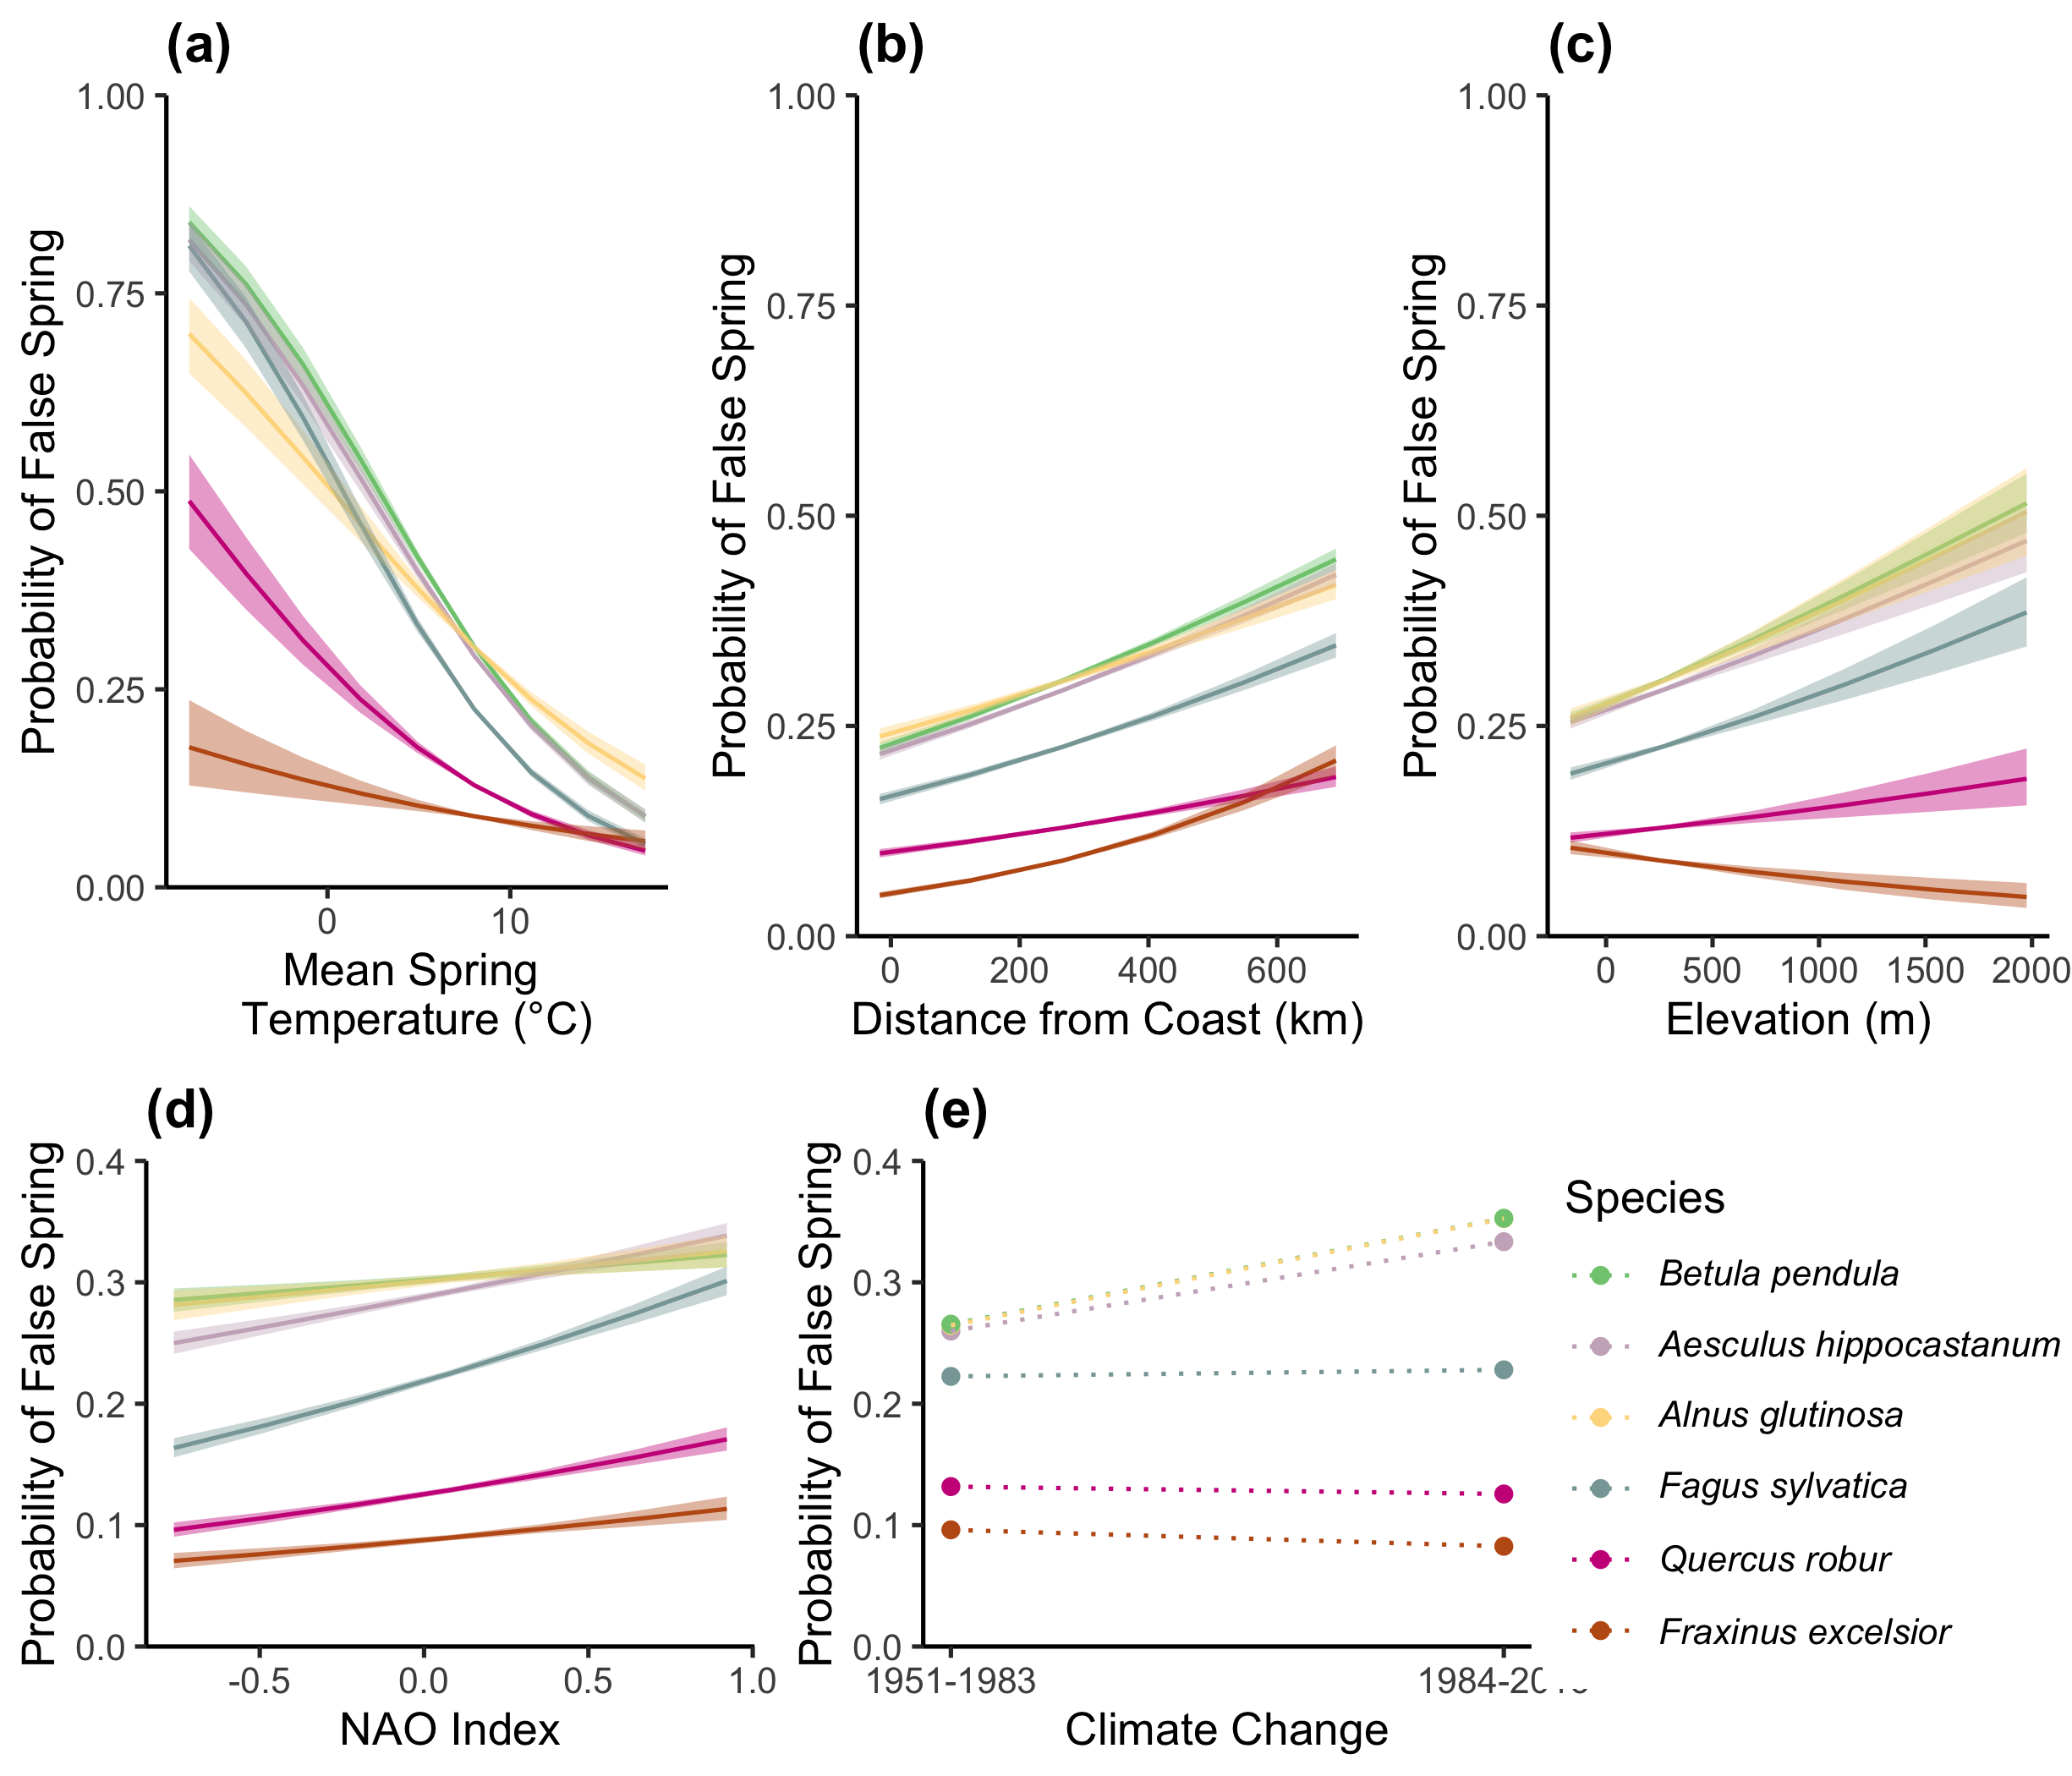
\includegraphics[width=16cm]{..//analyses/figures/InteractionPlots/Species_orig.png}
  -\caption{Species-level variation across geographic and spatial predictors (i.e., mean spring temperature (\textbf{a}), distance from the coast (\textbf{b}), elevation (\textbf{c}), and NAO index (\textbf{d})). Lines and shading are the mean and 98\% uncertainty intervals for each species. To reflect the raw data, we converted the model output back to the original scale for the x-axis in each panel. See Table \ref{tab:suppmodorig} for full model output. }\label{fig:spp}
  -\end{center}
  -\end{figure}}



\end{document}
